
The experiment setup is described in~\cref{ssec:setup}. 
We present performance results with production data in~\cref{ssec:prod} and with standard synthetic workloads in~\cref{ssec:synthetic}. 

The baseline for our evaluation is RocksDB -- a mature and widely-used industrial KV-store. 
We use the recent RocksDB release 5.17.2, available Oct 24, 2018.  It is worth noting that RocksDB's performance 
is significantly improved  in this release~\cite{CallaghanCompaction}.   
In~\cref{ssec:pebbles} we compare \sys\ against PebblesDB~\cite{PebblesDB}, a research LSM prototype, and TokuDB~\cite{TokuDB} 
-- the only publicly available KV-store whose design is inspired by B$^\epsilon$-trees. Both  perform significantly worse than RocksDB and \sys, 
motivating our focus on RocksDB.


 
\subsection{Setup}
\label{ssec:setup} 

\paragraph{Methodology.} 
Our hardware is a 12-core (24-thread) Intel Xeon 5  with 4TB SSD disk.  
We run each experiment within a Linux container with 16GB RAM. 
Data is stored uncompressed.
We run 5 experiments for each data point and present the median measurement to eliminate outliers. Since experiments are long, the results vary 
little across runs. In all of our experiments, the STD was within $6.1\%$ of the mean, and in most of them below $3\%$. 

We employ a C++ implementation~\cite{Cpp-YCSB} of YCSB~\cite{YCSB}, the  standard  
benchmarking platform for KV-stores. YCSB provides a set of APIs and a synthetic workload suite inspired 
by real-life applications. In order to exercise production workloads, we extend YCSB to replay log files.
 
In each experiment, a pool of concurrent worker threads running identical
workloads stress-tests the KV-store. We exercise 12 YCSB workers 
and allow the data store to use 4 additional background threads for maintenance.
We also experimented with different numbers of worker threads, finding similar scalability trends in RocksDB and 
\sys; these results are omitted for lack of space.


\paragraph{Configuration.} 
To avoid over-tuning, all experiments use the data stores' default configurations. For RocksDB, we use the configuration exercised by its public 
performance benchmarks~\cite{RocksDBPerf}. 
We also experimented with tuning RocksDB's memory resources based on its performance guide~\cite{RocksDBMemoryTuning}; 
this had mixed results, improving performance by at most 25\% over the default configuration in some workloads but 
deteriorating it by up to 25\% in others. Overall, the default configuration performed best. 
We fixed the PebblesDB code to resolve a data race reported in the project's repository~\cite{pebbles-git-issue}. 

\sys's default configuration 
allocates 8GB to munks and 4GB to the row cache,
so together they consume 12GB out of the 16GB container. 
The row cache consists of three hash tables.  
The Bloom filters for funks are partitioned 16-way.  
We set the \sys\/ maximum chunk size limit to 10MB, the rebalance size trigger to 7MB, 
the funk log size limit to 2MB for munk-less chunks, and to 20MB for chunks with munks. 
The results of the experiments we ran in order to tune these parameters are omitted due to lack of space.

We focus on asynchronous persistence,  i.e., flushes to disk happen in the background; 
(with synchronous I/O, performance is an order-of-magnitude slower, trivializing the results 
in all scenarios that include puts). 

\subsection{Production data}
\label{ssec:prod}


\begin{figure*}[tb]
\centering
\begin{subfigure}{0.29\linewidth}
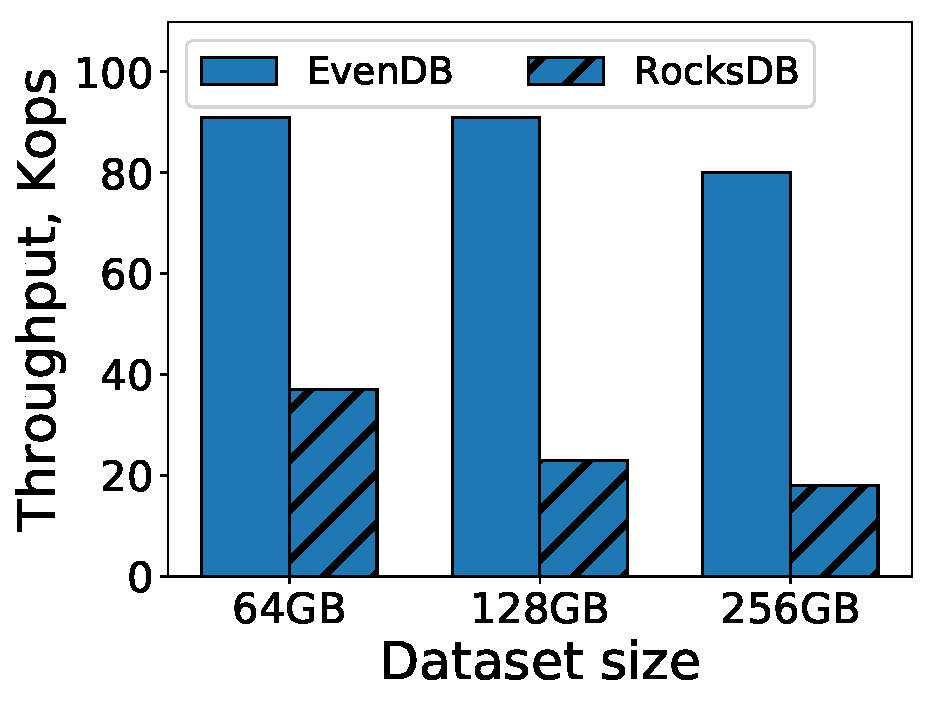
\includegraphics[width=\textwidth]{figs/ingestion.pdf}
\caption{Throughput, Kops}
\label{fig:prod:ingestion:a}
\end{subfigure}
\hspace{0.03\linewidth} 
\begin{subfigure}{0.29\linewidth}
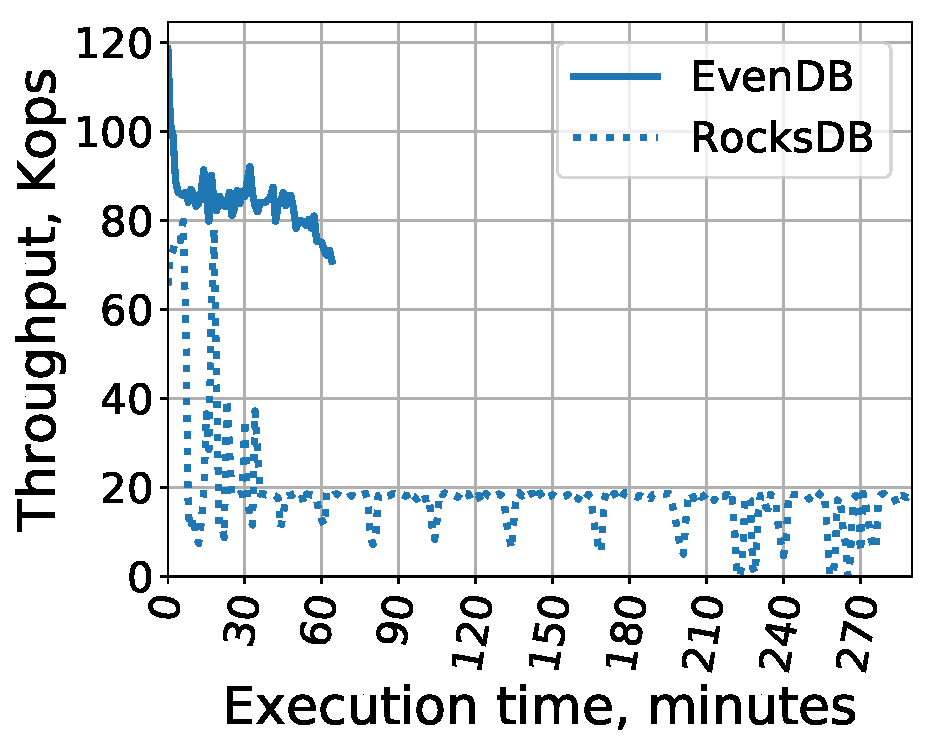
\includegraphics[width=\textwidth]{figs/throughput_256_ingestions_line.pdf}
\caption{Throughput dynamics, 256GB}
\label{fig:prod:ingestion:b}
\end{subfigure}
\hspace{0.03\linewidth} 
\begin{subfigure}{0.29\linewidth}
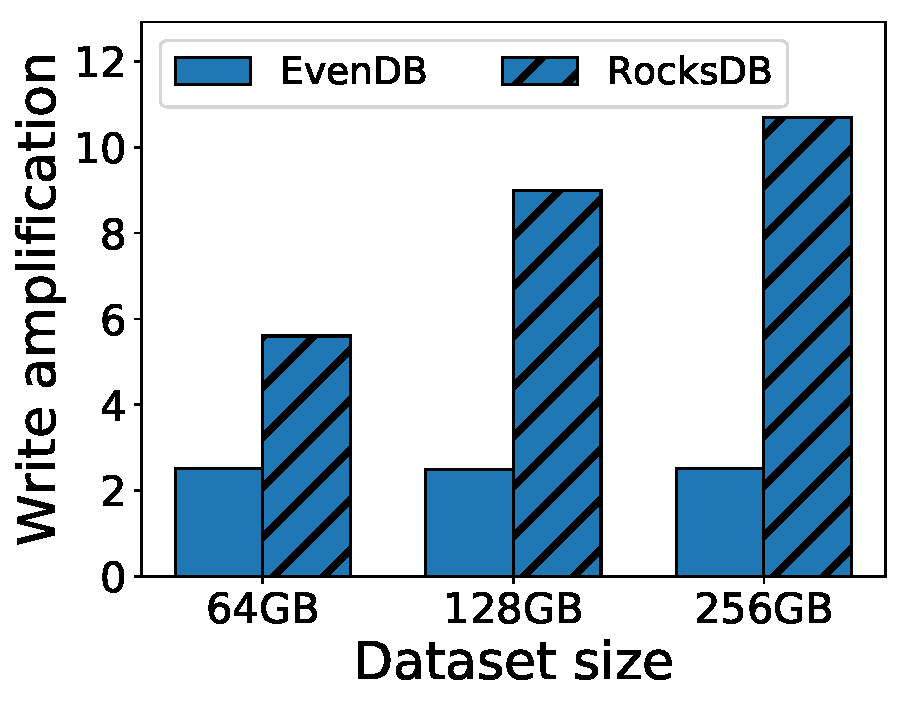
\includegraphics[width=\textwidth]{figs/write_amp_256.pdf}
\caption{Write amplification}
\label{fig:prod:ingestion:c}
\end{subfigure}
\caption{\sys\/ vs RocksDB performance under ingestion (100\% put) workload with production datasets.}
\label{fig:prod:ingestion}
\end{figure*}

\begin{figure*}[tb]
\centering
\begin{subfigure}{0.29\linewidth}
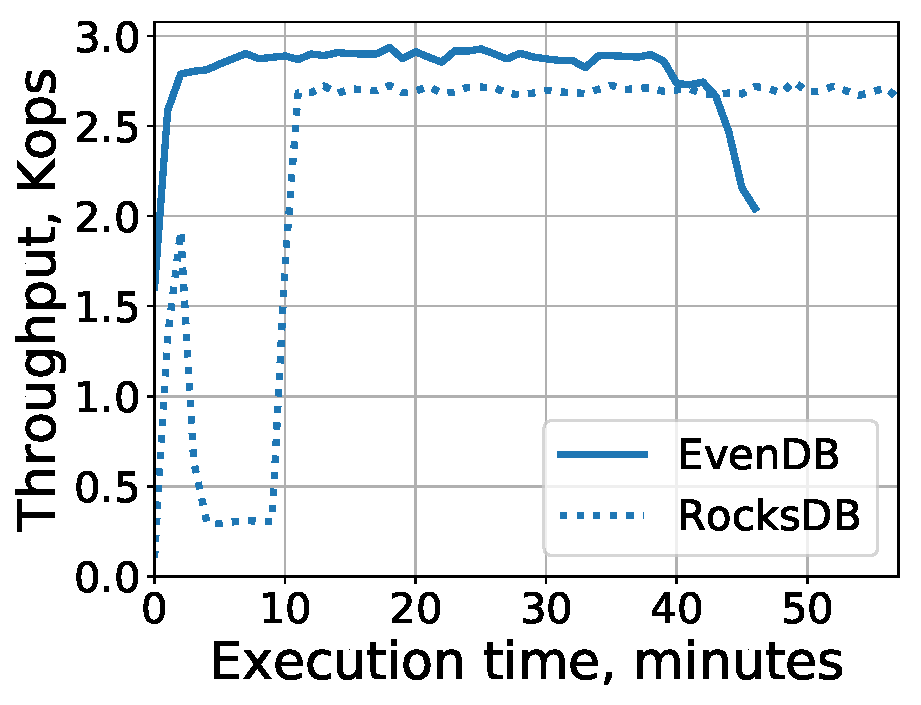
\includegraphics[width=\textwidth]{figs/throughput_64_scans_10s_line.pdf}
\caption{64 GB dataset}
\label{fig:prod:analytics:a}
\end{subfigure}
\hspace{0.03\linewidth} 
\begin{subfigure}{0.29\linewidth}
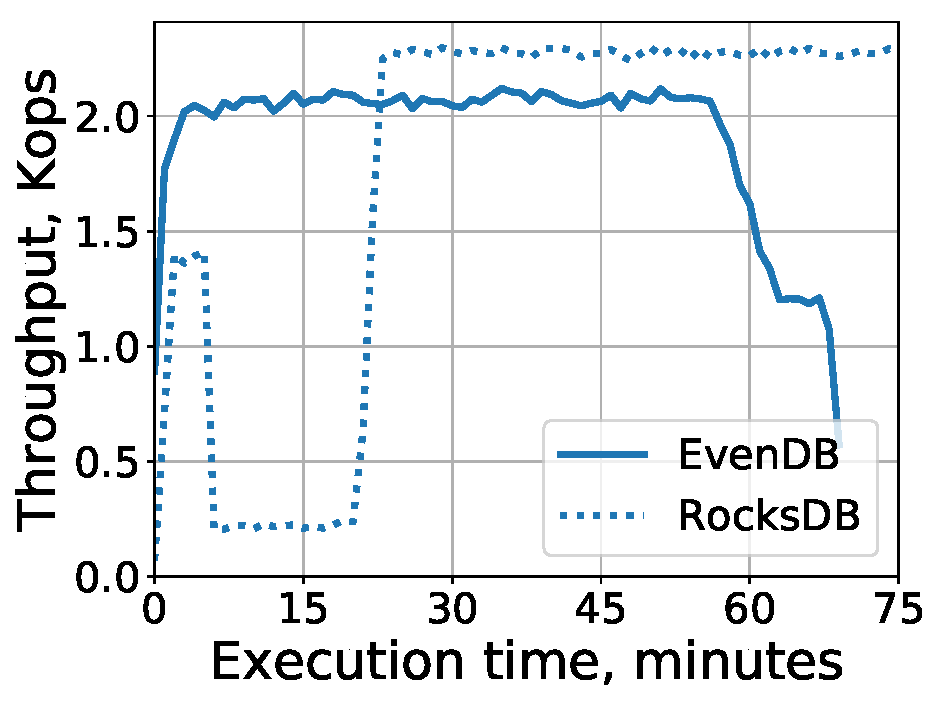
\includegraphics[width=\textwidth]{figs/throughput_128_scans_10s_line.pdf}
\caption{128 GB dataset}
\label{fig:prod:analytics:b}
\end{subfigure}
\hspace{0.03\linewidth} 
\begin{subfigure}{0.29\linewidth}
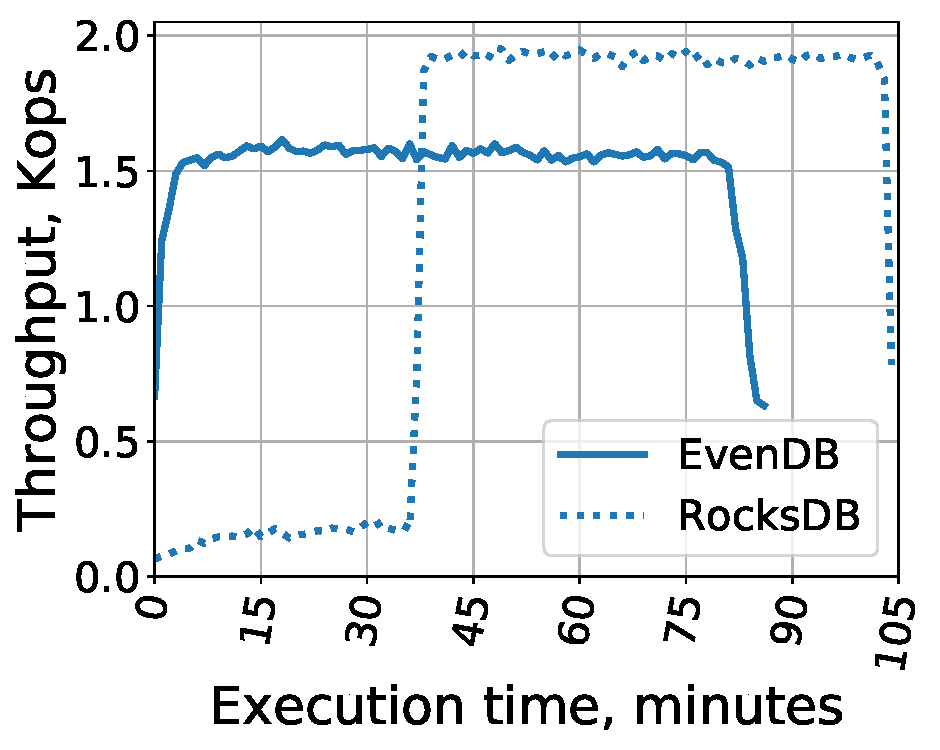
\includegraphics[width=\textwidth]{figs/throughput_256_scans_10s_line.pdf}
\caption{256 GB dataset}
\label{fig:prod:analytics:c}
\end{subfigure}
\caption{\sys\/ vs RocksDB throughput dynamics,  scan-dominated (95\% scans/5\% put) workload with production data.}
\label{fig:prod:analytics}
\end{figure*}



Our first set of experiments is driven by a log collected by a production mobile analytics engine. The log captures 
a stream  of $\sim$13M unique events per minute, with an average log record size of 800B, i.e., $\sim$10GB/min. 
We load the logged events into a table indexed by app id and timestamp. 
As noted in~\cref{sec:intro}, the app id distribution is heavy-tailed, i.e., the data exhibits spatial locality. 
We use this log to drive \emph{put-only} (100\% put) and \emph{scan-dominated} 
(95\% scan, 5\% put) tests.

\paragraph{Put-only (data ingestion).} 
\Cref{fig:prod:ingestion} presents our  data ingestion results. 
Here, we load 64GB, 128GB and 256GB of data, in timestamp order; note that this order is different from the KV-store's primary key. 
 \Cref{fig:prod:ingestion:a} depicts the throughput in each experiment. Clearly, \sys\/ is much faster than RocksDB and its advantage 
becomes more pronounced as the dataset grows. For example, \sys\/ ingests 256GB  within 1.1 hours, 
whereas RocksDB requires 4.85 hours (4.4x slower). Figure~\ref{fig:prod:ingestion:b} depicts the  
throughput dynamics for the 256GB dataset. RocksDB's throughput, while stable overall, suffers from stalls 
(lasting a minute or longer) caused by compactions. 
%\sys's throughput is noisier, because munk rebalances are more frequent than munk compactions; 
\sys\ delivers predictable performance, with a throughput constantly above 4x RocksDB's average rate.

Figure~\ref{fig:prod:ingestion:c} shows the write amplification in the same benchmark. 
While \sys's amplification is unaffected by  scaling, RocksDB deteriorates as the dataset (and consequently, the number of LSM levels) grows. 
%For example, for 256GB RocksDB's amplification factor is 10.7x, whereas \sys's is only 2.5x. 
These results underscore the importance of \sys's in-memory compactions, which consume CPU 
but dramatically reduce the I/O load by minimizing on-disk compaction (funk rebalances). 

This dichotomy between CPU and I/O usage can be observed in 
Table~\ref{fig:io_cpu_bound}, which summarizes  the overall resource consumption in the  256GB ingestion
experiment. We see that \sys\/ is CPU-intensive -- it exploits 40\% more CPU cycles than RocksDB, which means that its average CPU rate is 6.3x higher. 
On the other hand, RocksDB is I/O-intensive -- it reads 43x (!) more data than \sys\/ (recall that the workload is write-only; reading is for compaction purposes). 

\begin{table}[t]
\small
\begin{tabular}{lllll}
%\hline 
& Duration
 &  CPU time  & Read I/O & Write I/O\\
\hline 
\sys &  1.1 hr & 14.6 hr & 	47.6 GB 	&  645.2	GB \\
RocksDB & 4.85 hr & 10.4 hr &  2053.5 GB & 2660.4	GB\\
%\hline 
\end{tabular}
\caption{\sys\/ vs RocksDB resource consumption during ingestion (100\% put) of a 256GB production dataset.}
\label{fig:io_cpu_bound}
\end{table}



%Indeed, \sys\/ exploits  the workload's spatial locality, and spends most of its time handling RAM-resident data; it hardly 
%ever reads from disk (only upon funk rebalances, which are infrequent). RocksDB, on the other hand, spends a large fraction of its time in 
%compactions, which are insensitive to locality; it re-reads and re-writes the same data many times. 

\begin{figure*}[tb]
\centering
\begin{subfigure}{0.32\linewidth}
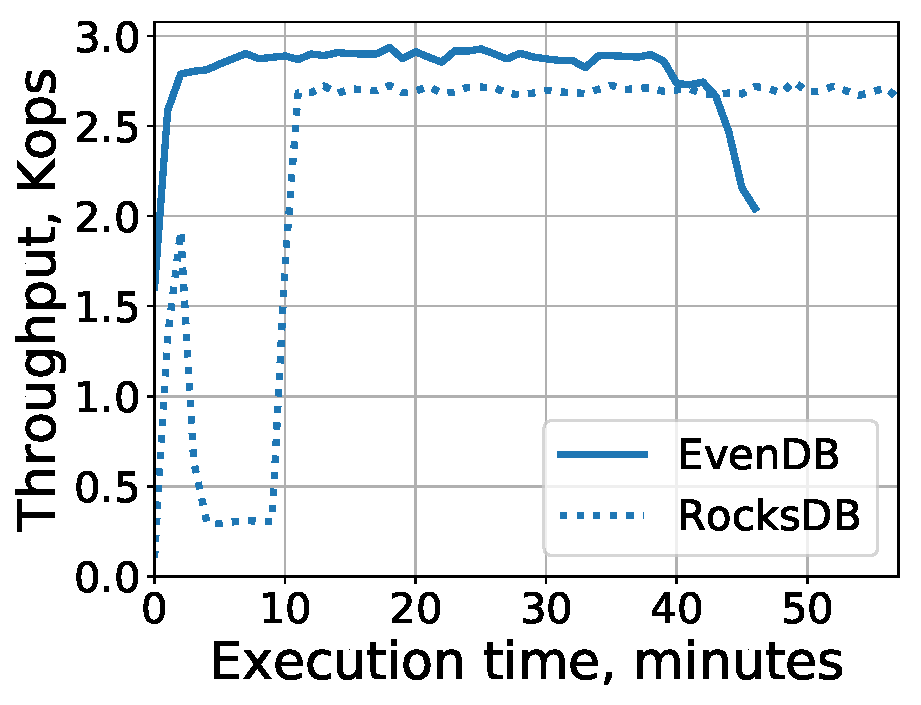
\includegraphics[width=\textwidth]{figs/throughput_64_scans_10s_line.pdf}
\caption{64 GB dataset}
\label{fig:prod:analytics:a}
\end{subfigure}
%\hspace{0.03\linewidth} 
\begin{subfigure}{0.32\linewidth}
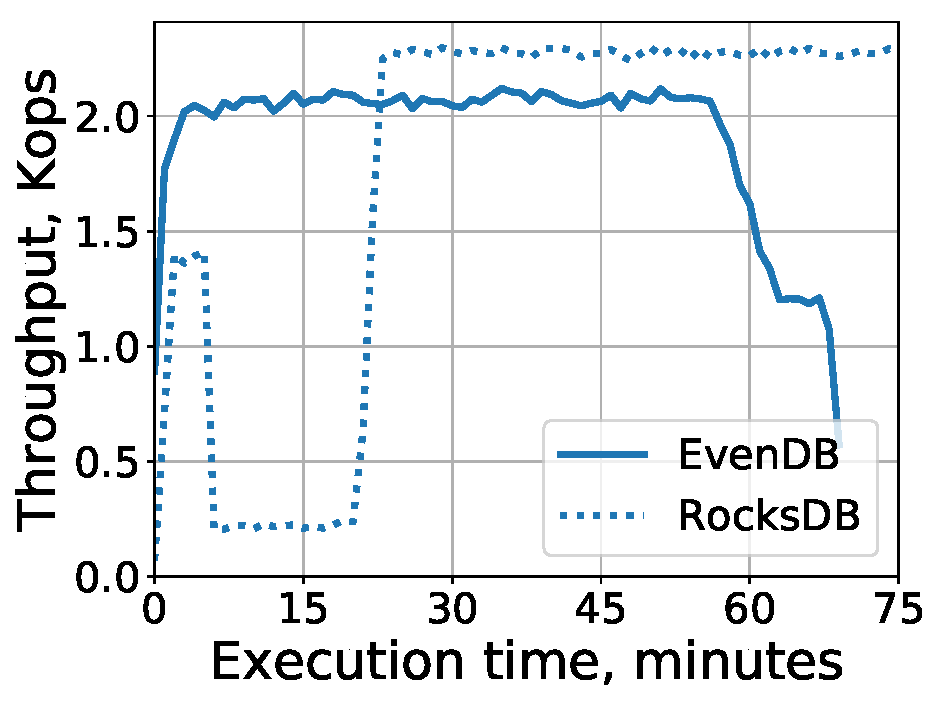
\includegraphics[width=\textwidth]{figs/throughput_128_scans_10s_line.pdf}
\caption{128 GB dataset}
\label{fig:prod:analytics:b}
\end{subfigure}
%\hspace{0.03\linewidth} 
\begin{subfigure}{0.32\linewidth}
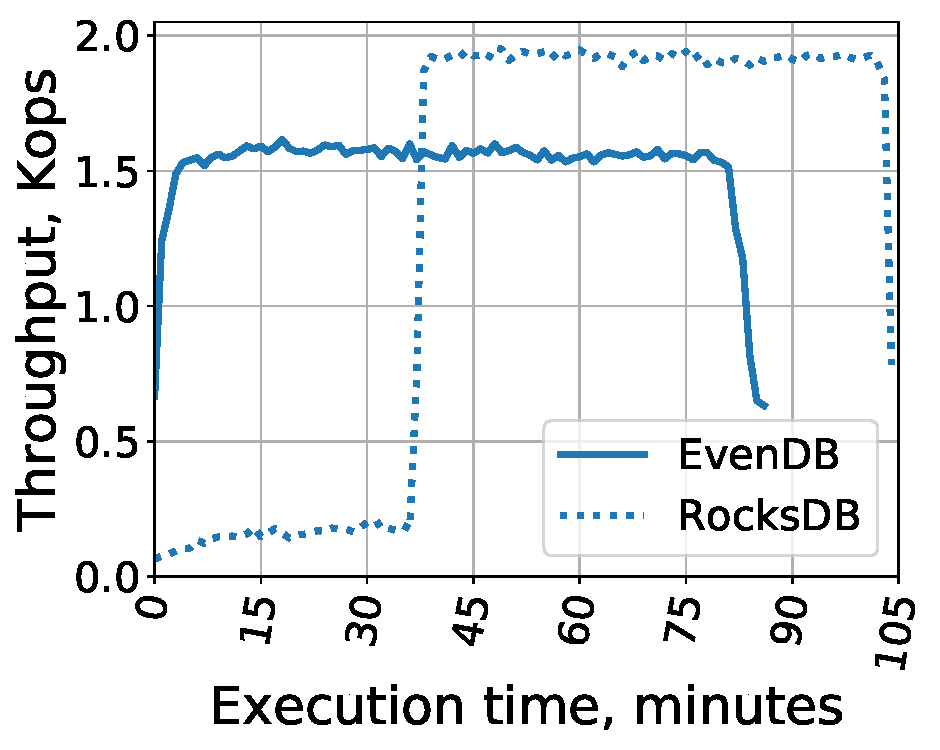
\includegraphics[width=\textwidth]{figs/throughput_256_scans_10s_line.pdf}
\caption{256 GB dataset}
\label{fig:prod:analytics:c}
\end{subfigure}
\caption{\sys\/ vs RocksDB throughput dynamics,  scan-dominated (95\% scans/5\% put) workload with production data.}
\label{fig:prod:analytics}
\end{figure*}

\paragraph{Scan-dominated (analytics).} We run 40M operations -- 95\% range queries, 5\% puts -- 
on the KV-store produced by the ingestion tests.
Every query scans a sequence of recent events within one app (all the scanned rows 
share the  app id key prefix).  
%We study short, medium, and long scans, covering 1 s, 10 s, and 1 min of the app's event history. 
The app id is sampled from the data distribution (so popular apps are queried more frequently).  
Figure~\ref{fig:prod:analytics} depicts the performance dynamics for queries that scan 1-minute histories.
We experimented also with shorter scans, with similar results, which are omitted for lack of space.

\sys\/ completes all experiments 20\% to 30\% faster than RocksDB. 
Yet the two systems' executions are very different. \sys's throughput stabilizes 
almost instantly upon transition from ingestion to analytics because its working set munks are already 
in memory. In contrast, it takes RocksDB 10 to 35 minutes (!) to reach the steady-state performance. 
During this period, it goes through multiple compactions, which degrade its application-level throughput 
beyond 90\%. 

After all compactions are done, RocksDB's improved organization gives it an advantage  over \sys\
(in large datasets) by up to 23\%, because \sys\ searches
in  logs of unpopular funks. We note that this tradeoff between the maintenance cost (for compaction) 
and the scan performance after maintenance  can be controlled via \sys's log size limit parameter.
(E.g., we saw that scan throughput can  grow by up to 20\%  by tuning the system to use 512KB logs instead of
the default 2MB; this experiment is omitted for lack of space.)

%In the long run, %\sys\/ and RocksDB exhibit similar performance under this workload, 
%\inred{RocksDB's performance exceeds \sys's with the large 
%with an eventual advantage to RocksDB in long executions with a large dataset. 
%However, the  dynamics are different.




\subsection{Synthetic benchmarks}
\label{ssec:synthetic} 


In this section, we closely follow the YCSB benchmarking methodology. 
Each experiment first  loads a sequence of KV-pairs, ordered by key, to an initially empty store, then  
runs read operations to warm the caches, and then exercises -- and measures --  the specific experiment 
scenario. Experiments perform 80M data accesses (fewer if some of them are scans). 
Since the load is in key order, the data stores are sorted from the outset, and RocksDB's files cover disjoint key ranges. 
This reduces the overhead of compaction and mitigates the stabilization delay observed in~\cref{ssec:prod}.  Thus, 
performance remains stable throughout the measurement period.

\subsubsection{Workloads}
%\paragraph{Workloads.} 

We vary the dataset size from 4GB to 64GB in order to test multiple locality 
scenarios with respect to the available 16GB of RAM. Similarly to the published RocksDB benchmarks~\cite{RocksDBPerf}, 
the keys are 32-bit integers in decimal encoding (10 bytes), which YCSB pads with a 4-byte prefix (so effectively, 
the keys are 14 byte long). Values are 800-byte long. 


% A synthetic workload is defined by  (1)  ratios of get, put, and scan accesses, and (2) a distribution of key access frequencies. 
\noindent
We study the following four key-access distributions:  

%\begin{description}
%\item [Zipf-simple] 
\emph{1. Zipf-simple} -- the standard YCSB Zipfian distribution over simple (non-composite) keys. 
Key access frequencies are sampled from a Zipf distribution 
(following~\cite{Gray:1994:QGB:191839.191886}), with $\theta = 0.8$
(the most popular key's frequency is  $\sim 0.7\%$). 
The ranking is over a random permutation of the key range, so popular keys are uniformly dispersed. % (no spatial locality).
% The key locations are sampled uniformly at random from the whole data range. 
%This workload exhibits medium temporal locality (e.g., the most popular key's frequency is approximately $0.7\%$) and no spatial locality. 
%This is a standard YCSB workload that captures a multitude of use cases  -- e.g., a web page cache distribution by URL. 

%\item [Zipf-composite]  
\emph{2. Zipf-composite} -- a Zipfian distribution over composite keys.
The key's $14$ most significant bits comprise the primary attribute, which  
is drawn from a Zipf ($\theta=0.8$) distribution over its range. The remainder of the key is drawn uniformly at random.
We also experimented with a Zipfian distribution of the key's suffix and 
the trends were similar. %, since performance is most affected by  the primary dimension.
%'s distribution. %Zipf-composite exhibits high spatial locality.% it represents workloads 
%with composite keys.%, such as message threads~\cite{Borthakur:2011:AHG:1989323.1989438},
%social network associations~\cite{Armstrong:2013:LDB:2463676.2465296}, and analytics databases~\cite{flurry},
%and other scenarios with spatial locality of keys, e.g.,  reverse URL domains.

%\item [Latest-simple] 
\emph{3. Latest-simple} -- a standard YCSB workload reading simple keys from a distribution skewed towards recently added ones. 
Specifically, the sampled key's position wrt the most recent key is distributed Zipf. 
%This is with medium spatial and temporal locality, modeling e.g., status updates.

%\item [Uniform] 
\emph{4. Uniform} -- ingestion of keys sampled uniformly at random. RocksDB
reports a similar benchmark~\cite{rocksdb-benchmarks}. %; we present it for completeness.
%\end{description}

The workloads exercise different mixes of puts, gets, and scans. We use standard YCSB scenarios 
(A to F) that range from write-heavy ($50\%$ puts) to read-heavy ($95\%-100\%$ gets or scans). 
%In order to stress the system even more on the write side,
We also introduce a new workload, P, comprised of $100\%$ puts (a data ingestion scenario
as in~\cref{ssec:prod}).
%non-sequential data load scenario (e.g., an ETL from an external data pipeline~\cite{flurry}). 

\subsubsection{Evaluation results}

\begin{figure*}[tb]
\centering
\begin{subfigure}{0.32\linewidth}
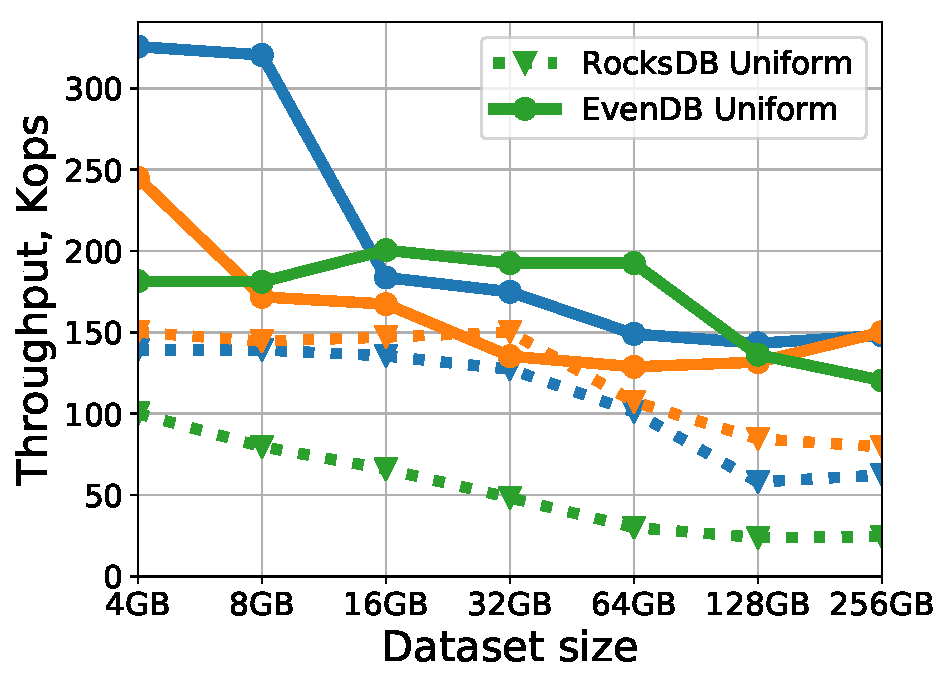
\includegraphics[width=\textwidth]{figs/Workload_P_line.pdf}
\caption{P -- 100\% put}
\label{fig:throughput:p}
\end{subfigure}
%\hspace{0.01\linewidth} 
\begin{subfigure}{0.32\linewidth}
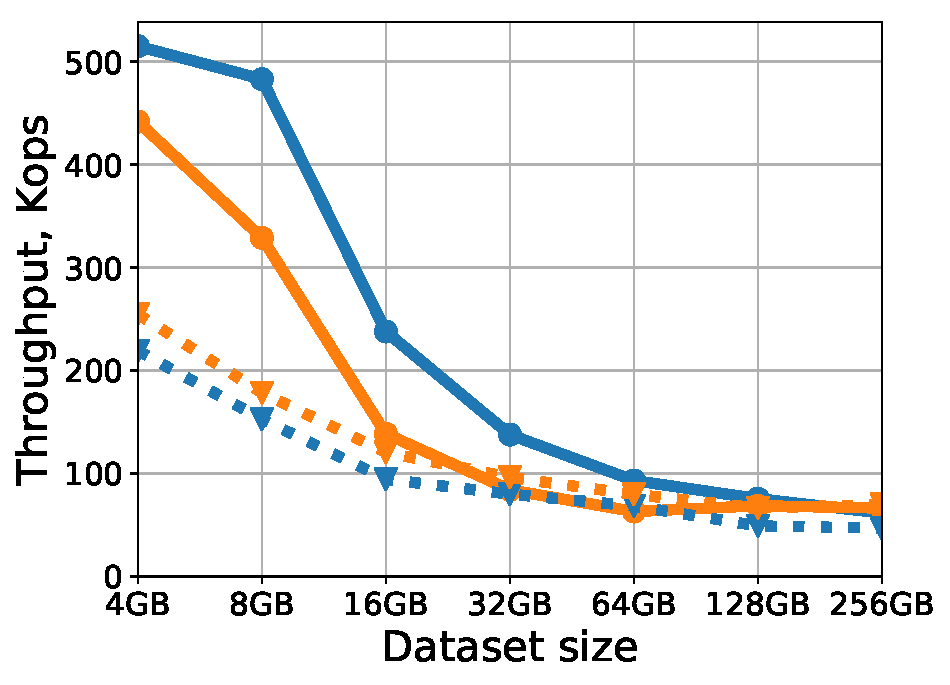
\includegraphics[width=\textwidth]{figs/Workload_A_line.pdf}
\caption{A -- 50\% put, 50\% get}
\label{fig:throughput:a}
\end{subfigure}
%\hspace{0.01\linewidth} 
\begin{subfigure}{0.32\linewidth}
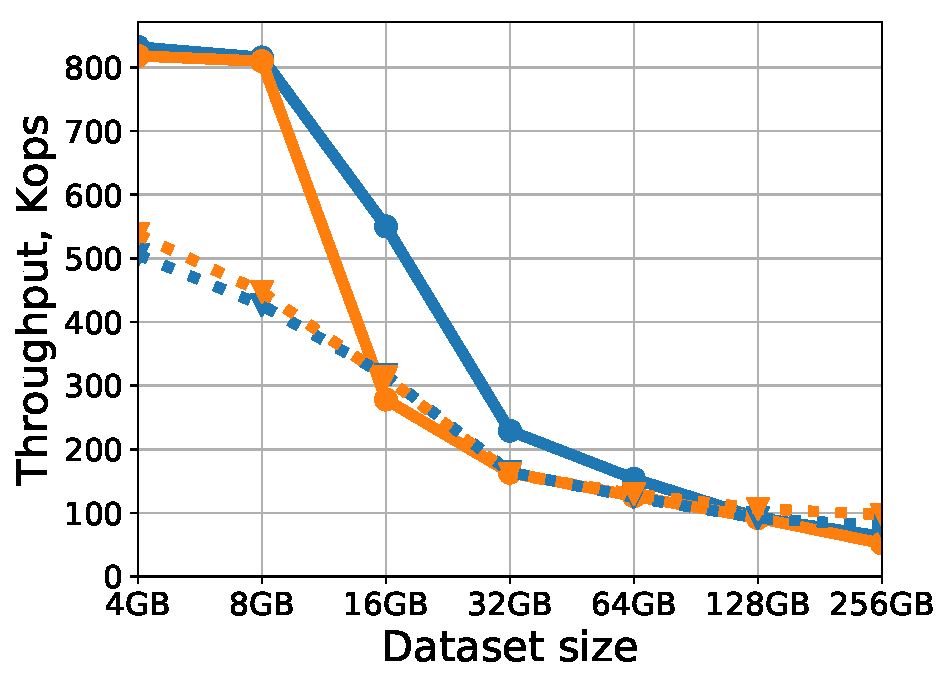
\includegraphics[width=\textwidth]{figs/Workload_B_line.pdf}
\caption{B -- 5\% put, 95\% get}
\label{fig:throughput:b}
\end{subfigure}
%\hspace{70pt}
\begin{subfigure}{0.32\linewidth}
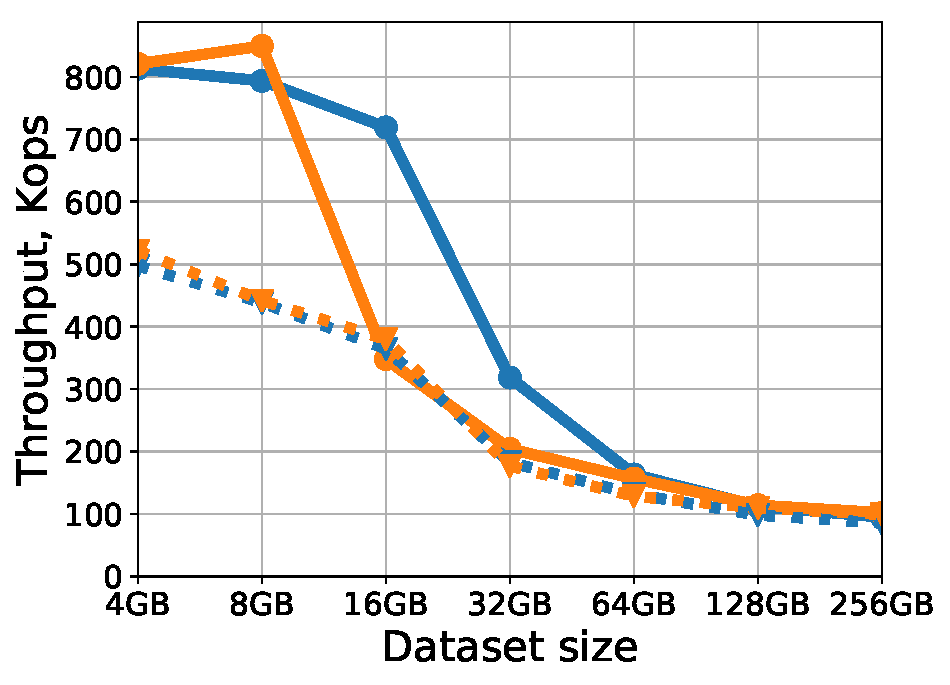
\includegraphics[width=\textwidth]{figs/Workload_C_line.pdf}
\caption{C -- 100\% get}
\label{fig:throughput:c}
\end{subfigure}
\begin{subfigure}{0.32\linewidth}
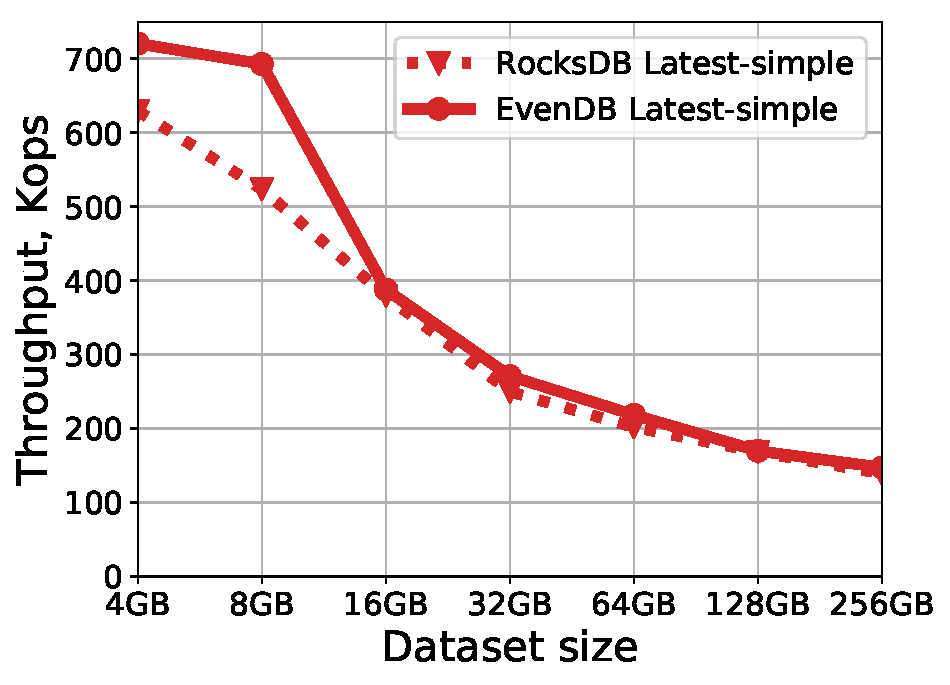
\includegraphics[width=\textwidth]{figs/Workload_D_line.pdf}
\caption{D -- Latest-simple, 5\% put, 95\% get}
\label{fig:throughput:d}
\end{subfigure}
\begin{subfigure}{0.32\linewidth}
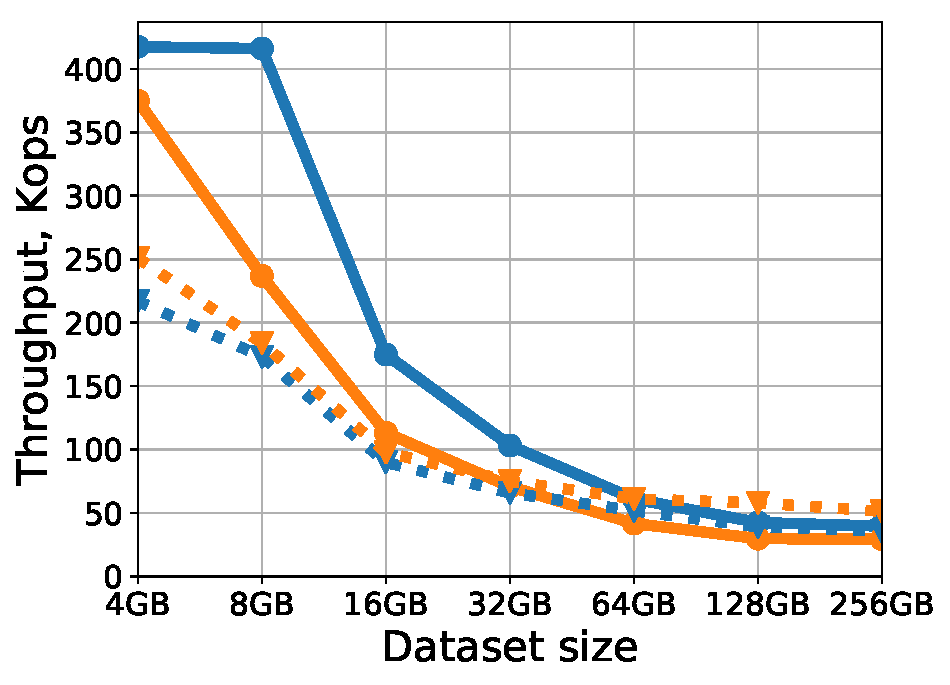
\includegraphics[width=\textwidth]{figs/Workload_F_line.pdf}
\caption{F -- 100\% get-modify-put}
\label{fig:throughput:f}
\end{subfigure}
%\hspace{70pt}
\begin{subfigure}{0.32\linewidth}
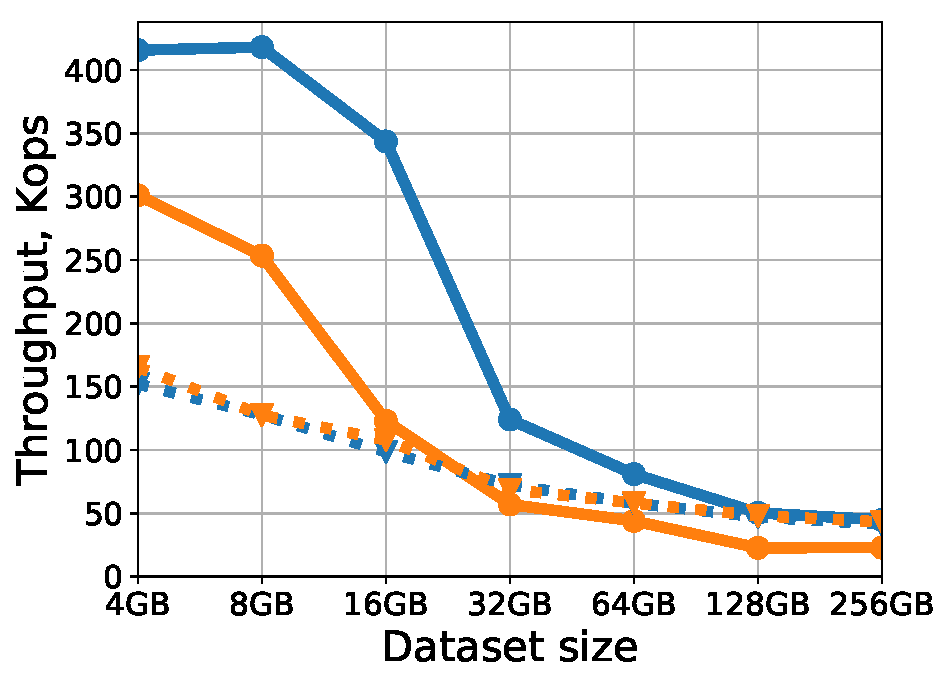
\includegraphics[width=\textwidth]{figs/Workload_E-_line.pdf}
\caption{E10 \\ 5\% put, 95\% scan (10 rows)}
\label{fig:throughput:e10}
\end{subfigure}
\begin{subfigure}{0.32\linewidth}
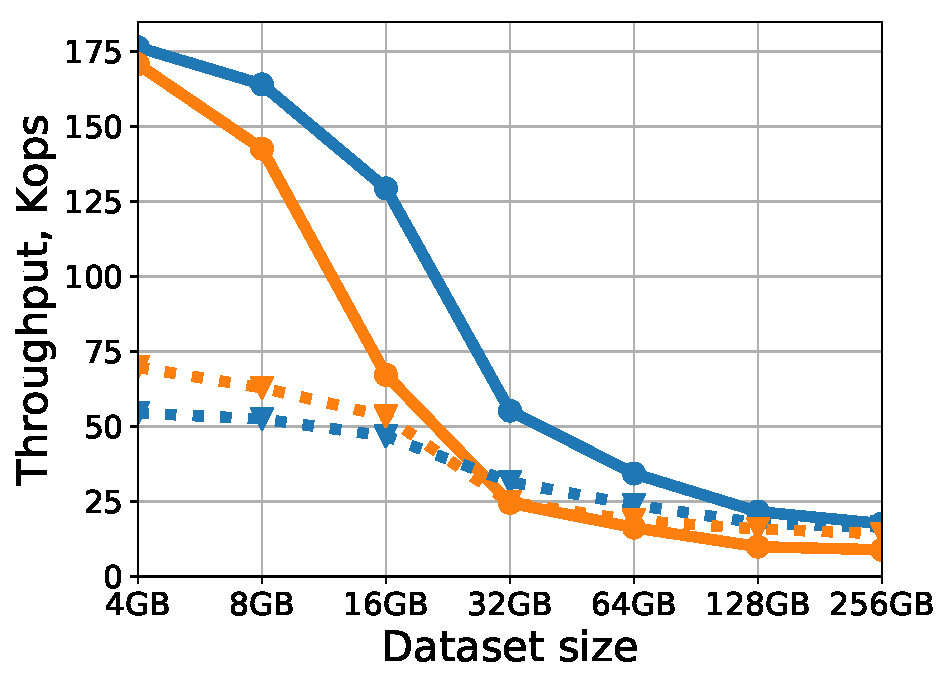
\includegraphics[width=\textwidth]{figs/Workload_E_line.pdf}
\caption{E100 \\ 5\% put, 95\% scan (100 rows)}
\label{fig:throughput:e100}
\end{subfigure}
\begin{subfigure}{0.32\linewidth}
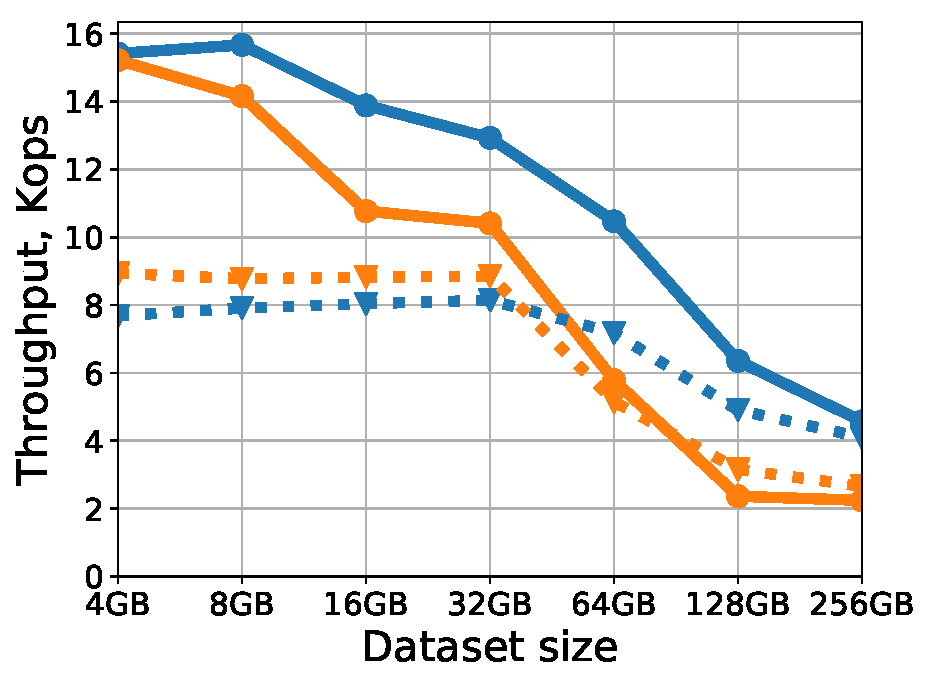
\includegraphics[width=\textwidth]{figs/Workload_E+_line.pdf}
\caption{E1000 \\5\% put, 95\% scan (1000 rows)}
\label{fig:throughput:e1000}
\end{subfigure}
\begin{subfigure}{\linewidth}
\centerline{

\includegraphics[width=0.9\textwidth]{figs/legend.pdf}
\vspace{-5mm}
}
\end{subfigure}
\caption{
{\sys\/ vs RocksDB throughput under YCSB workloads with various key distributions.}
}
\label{fig:throughput}
\end{figure*}

Figure~\ref{fig:throughput} presents the throughput measurements in all YCSB workloads. 
Except for workload D, which exercises the Latest-simple pattern
(depicted in red), all benchmarks are run with both  Zipf-simple (orange) 
and Zipf-composite (blue). The P (put-only) workload 
additionally exercises the Uniform access pattern (green). \sys\/ results are depicted with solid
lines, and RocksDB with dotted lines.

We now discuss the results for the different scenarios.
  
\paragraph{ Put-only (data ingestion)} is tested in workload
{P} (100\% put, Figure~\ref{fig:throughput:p}). 
\sys's throughput is 1.8x to 6.4x that of RocksDB's with uniform keys, 1.3x to 2.3x with Zipf-composite keys, 
and 0.9x to 1.6x with Zipf-simple keys. This scenario's bottleneck is the reorganization of persistent data  
(funk rebalances in \sys, compactions in RocksDB), which causes write amplification and hampers performance. 
 
 Under the Zipf-composite workload, \sys\ benefits from spatial locality whereas RocksDB's write performance 
 is relatively insensitive to it, as is typical for LSM stores. For small datasets (4-8GB), \sys\/ accommodates 
all puts in munks, and so funk rebalances are rare. In big datasets, funk rebalances do occur, but mostly in 
munk-less chunks, which are accessed infrequently. This is thanks to \sys\/'s high log size limit for chunks 
with munks. Hence, in both cases, funk rebalances incur less I/O than RocksDB's compactions, 
which do not distinguish between hot and cold data. 

% Under the Zipf-simple workload, the gains are moderate due to the low spatial locality. They are most pronounced 
% for small datasets that fit into RAM.
 
The Uniform workload exhibits no locality of any kind. 
 \sys\/ benefits from this because keys are dispersed evenly across chunks, hence all funk logs grow 
 slowly, and funk rebalances are infrequent. The throughput is therefore insensitive to the dataset 
 size. In contrast, RocksDB performs compactions frequently albeit they are not effective (since there are few redundancies). Its throughput 
 degrades  with the data size since when compactions cover more keys they engage more files.
 

   
The write amplification in this experiment is summarized in 
Figure~\ref{fig:writeamp}. We see that \sys\/ reduces the disk write rate dramatically, 
with the largest gain observed for big datasets (e.g.,  for the 64GB dataset 
the amplification factors are $1.3$ vs $3.1$ under Zipf-composite, and $1.1$ vs $7.6$ under Uniform). 

\begin{figure}[t]
	\centering
	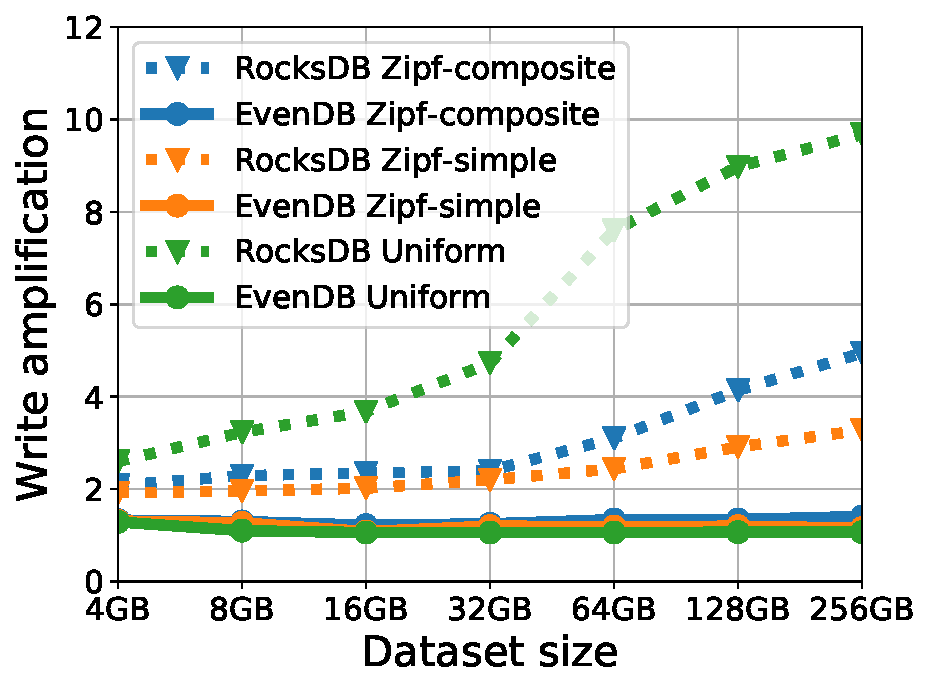
\includegraphics[width=0.4\textwidth]{figs/write_amp_p_line.pdf}
	\caption{{\sys\/ vs RocksDB write amplification under the put-only workload P.}}
	\label{fig:writeamp}
\end{figure}

\paragraph{ Mixed put-get} is represented in workloads A (50\% put, 50\% get, Figure~\ref{fig:throughput:a}) and 
F (100\% get-modify-put, Figure~\ref{fig:throughput:f}). Note that the latter exercises the usual get and put API (i.e., does not provide atomicity). 
In this scenario, \sys\ works well with composite keys, e.g., in workload A it  achieves $1.4$x to $3.5$x the throughput of RocksDB due to better exploitation of spatial locality. 
With simple keys, on the other hand, the get-put mix is particularly challenging for \sys, which serves many gets from disk due to the
low spatial locality. The bottleneck is the linear search in funk logs, which  fill
up due to the high put rate.
RocksDB's caching is more effective in this scenario, so its disk-access rate in get operations is lower,  resulting in faster gets. 
Note that \sys\/ is still reasonably close to RocksDB in the worst case 
(0.75x and 0.7x throughput for the 64GB dataset in A and F, respectively).
%(In-memory searches are three orders of magnitude faster.)

Figure~\ref{fig:tail_latency}, which depicts tail (95\%) put and get latencies in this scenario, 
corroborates our analysis. \sys\/ has faster puts and faster or similar get tail latencies with composite keys
(Figure~\ref{fig:tail_latency:co}). With simple keys (Figure~\ref{fig:tail_latency:si}),  
the tail put latencies are similar in the two data stores, but the tail get latency of \sys\ 
in large datasets surges.

 To understand this spike, 
we break down the get latency in  Figure~\ref{fig:readstat}. 
Figure~\ref{fig:readstat:dist} classifies gets by the storage  component 
that fulfills the request, and Figure~\ref{fig:readstat:lat} presents the disk search latencies by component. 
We see that with large datasets, disk access dominates the latency.
For example, in the 64GB dataset, $3.3\%$ of gets are served from logs under Zipf-composite vs $4\%$ under Zipf-simple,
and the respective log search latencies are $2.6$ ms vs $4.2$ ms. This is presumably because in the latter, puts are more dispersed, 
hence the funks are cached less effectively by the OS, and the disk becomes a bottleneck due to the higher I/O rate.



\begin{figure}[htb]
\centering
\begin{subfigure}{0.49\linewidth}
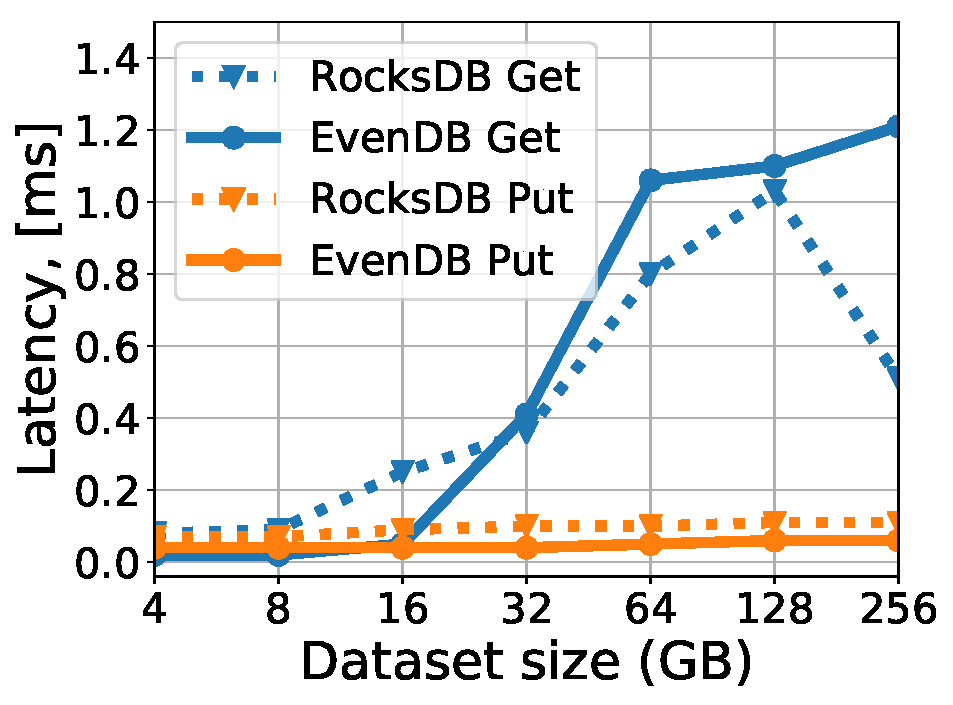
\includegraphics[width=\textwidth]{figs/tail_flurry_line.pdf}
\caption{Zipf-composite}
\label{fig:tail_latency:co}
\end{subfigure}
\begin{subfigure}{0.49\linewidth}
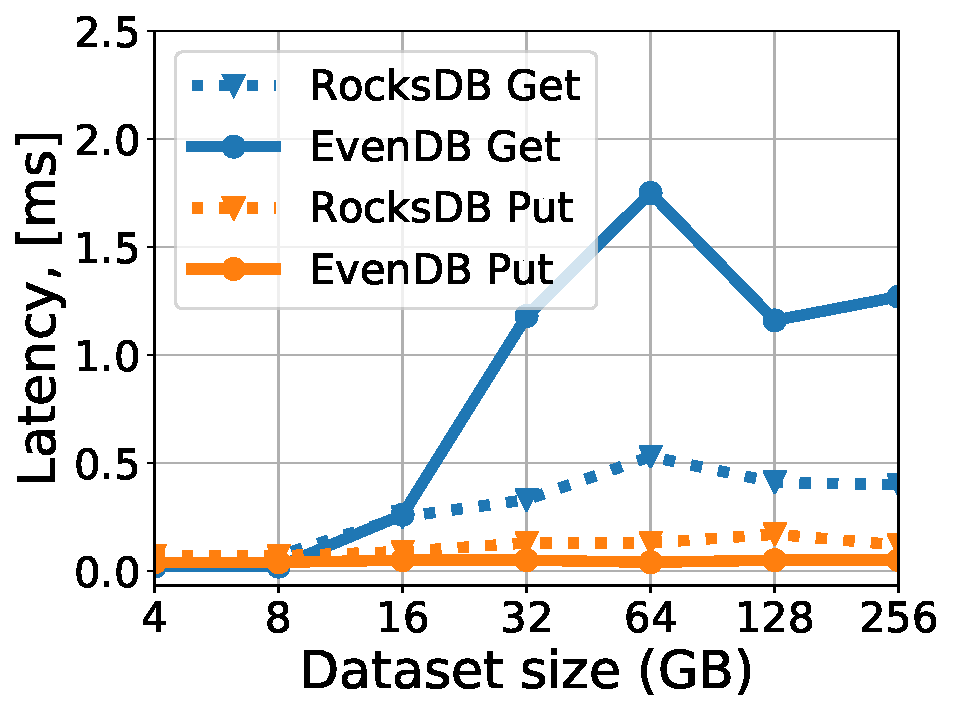
\includegraphics[width=\textwidth]{figs/tail_zipf_line.pdf}
\caption{Zipf-simple}
\label{fig:tail_latency:si}
\end{subfigure}
\caption{{\sys\/ vs RocksDB 95\% latency (ms), under a mixed get-put workload A.}}
\label{fig:tail_latency}
\end{figure}

\begin{figure}[htb]
\centering
%\hspace{0.05\linewidth}
\begin{subfigure}{0.6\linewidth}
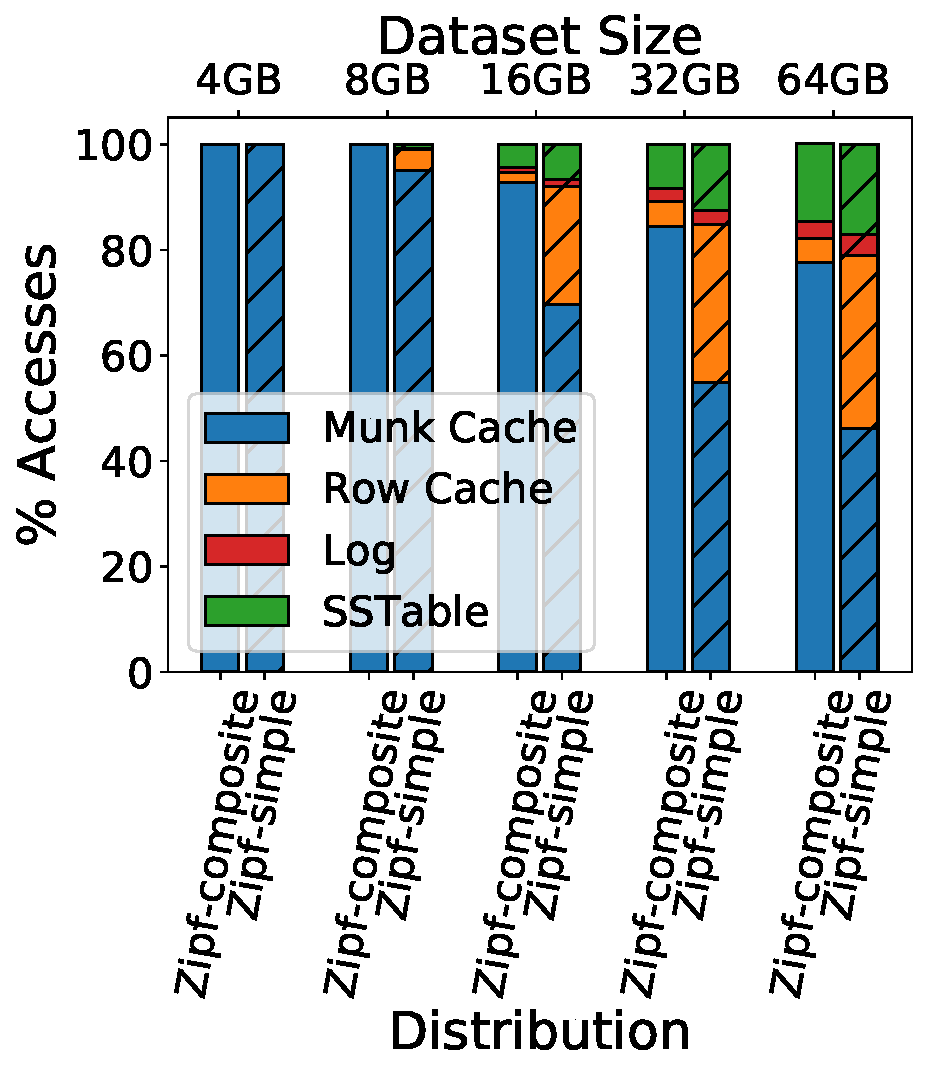
\includegraphics[width=\textwidth]{figs/Time_percentage_A.pdf}
\vskip .1in
\caption{Fraction of get accesses}
\label{fig:readstat:dist}
\end{subfigure}

%\hspace{0.05\linewidth}
\begin{subfigure}{0.6\linewidth}
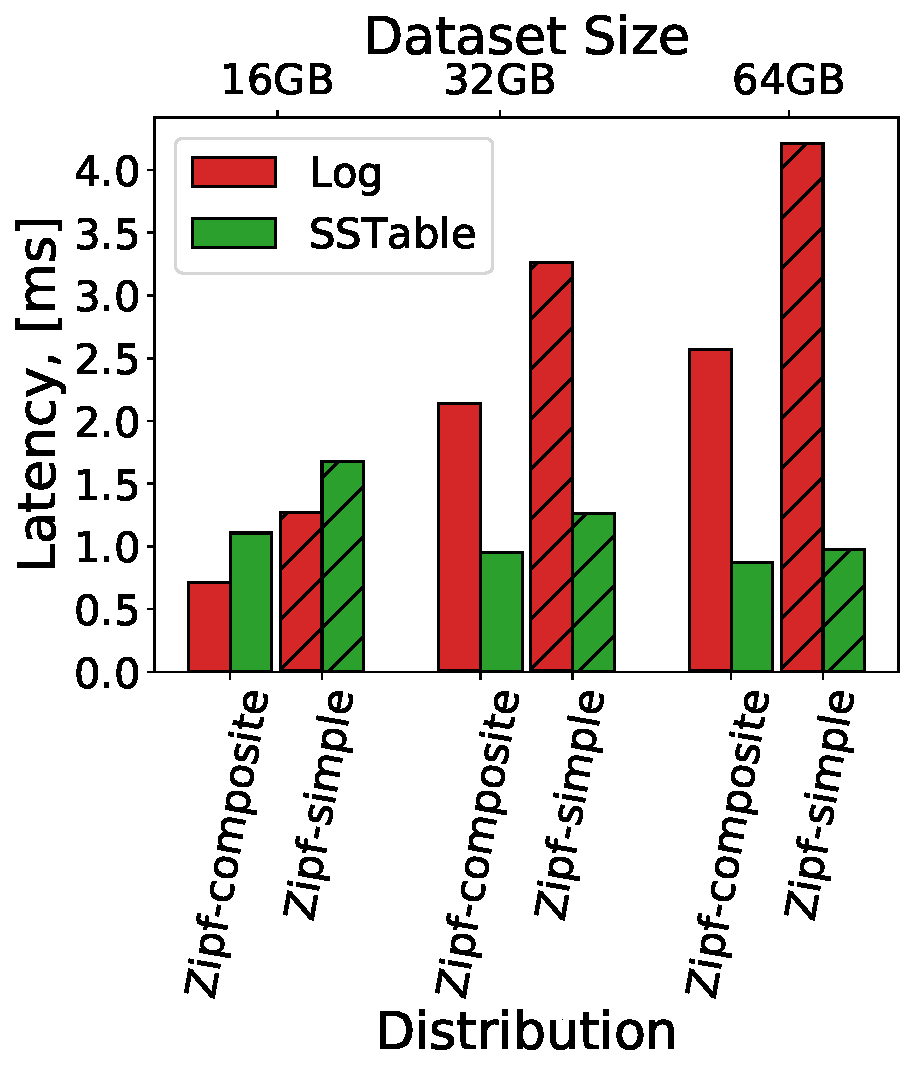
\includegraphics[width=\textwidth]{figs/Latency_A.pdf}
\caption{On-disk get access latency}
\label{fig:readstat:lat}
\end{subfigure}
\caption{{\sys\/ get latency breakdown by serving component, under a mixed get-put workload A.}}
\label{fig:readstat}
\end{figure}

The figure also shows that the row cache becomes instrumental as spatial locality drops -- it serves $32.8\%$ of gets with Zipf-simple 
vs $4.5\%$ with Zipf-composite. 

\paragraph{ Get-dominated} 
workloads (B--D, Figures~\ref{fig:throughput:b}--\ref{fig:throughput:d}) are 
favorable to 
\sys, which has a marked advantage in all key distributions with small datasets (up to the available RAM size) 
and also with Zipf-composite keys in large datasets. 
For example, in workload C (100\% get, Figure~\ref{fig:throughput:c}), 
\sys\/ performs $1.2$x to $2$x better than RocksDB with composite keys,
and up to $1.9$x  with simple ones (for small datasets). 
In these scenarios, \sys\  manages to satisfy most gets from munks, resulting in good performance.
RocksDB relies mostly on the OS cache to serve these requests and so it pays the overhead for invoking system calls. 
%As we discuss in~\S\ref{ssec:drill} below, 
RocksDB's performance in this scenario can be improved by 
using a larger application-level block cache,
but this hurts performance for bigger datasets as well as in other benchmarks.
(These results are not elaborated due to space limitations). 

\paragraph{ Scan-dominated} benchmarks (E10--1000,  5\% put, 95\% scan, Figures~\ref{fig:throughput:e10}-~\ref{fig:throughput:e1000})
iterate through a number of items 
sampled uniformly in the range [1,S], where S is  10, 100, or 1000. 
This workload (except with short scans on  large datasets) is favorable to \sys, 
since it exhibits the spatial locality the system has been designed for. 
Under Zipf-composite, \sys\/ achieves $1.4$x to $3.2$x throughput vs RocksDB.   
With simple keys, \sys\ improves over RocksDB when scans are long or the dataset is small. 
\sys's scan performance on big datasets can be improved by adapting the funk log size limit to this workload. 

\subsection{Additional KV-Stores}
\label{ssec:pebbles} 


We experimented with Percona TokuDB~\cite{TokuDBgit}; although deprecated, no newer version is available. 
The results were at least an order-of-magnitude slower than RocksDB across the board, and therefore we do not present them. 
Note that this is in line with previously published comparisons~\cite{DBLP:conf/cidr/DongCGBSS17,tucana,toku-rocks-inno}.
We did not compare \sys\/  against
% the MySQL default KV-store, 
InnoDB because the latter is not easily separable 
from the MySQL code. Yet previous evaluations have found  InnoDB to be inferior to both RocksDB and TokuDB under 
write-abundant workloads~\cite{toku-rocks-inno}.

We next compare \sys\ to PebblesDB, which was shown to significantly improve over RocksDB~\cite{PebblesDB},
mostly in single-thread experiments, before RocksDB's recent version was released.  
We compare \sys\ to PebblesDB in a challenging  scenario for \sys, with a 32GB dataset and the Zipf-simple key 
distribution. We run each YCSB workload with 1, 2, 4, 8 and 12 threads. The results are summarized in Table~\ref{fig:pebbels-throughput}. 
While PebblesDB is slightly faster on some single-threaded benchmarks, from 2 threads and onward \sys\ is consistently better in all experiments, 
with an average performance improvement of almost 1.8x.  In all benchmarks, 
 \sys's advantage grows with the level of parallelism. We observed a similar trend with smaller datasets. 

We note that in our experiments, RocksDB also consistently outperforms PebblesDB. 
The discrepancy with the results reported in~\cite{PebblesDB} 
can be attributed, e.g., to RocksDB's evolution, resource constraints (running within a 
container), a different hardware setting, and increased  parallelism.   

\begin{table}
\centering
{\small{
\begin{tabular}{cccccc}
%Workload & Zipf-simple & Zipf-composite \\
P & A & B, C & D& E10--1000 & F \\
\hline 
0.86--2.8x & 0.94--1.6x & 1.4--2.3x &  0.98-2x & 1.0--3.4x &  0.84-1.23x  \\
\end{tabular}
}}
\caption{{\sys\/ throughput improvement over PebblesDB, 32GB dataset, Zipf-simple keys, 1--12 worker threads.
\sys's advantage grows with the number of threads.}}
\label{fig:pebbels-throughput}
\end{table}

\subsection{Insights}
\label{ssec:drill} 








